\section{Analogue Output}
\setlength{\tabcolsep}{0pt}
\begin{center}
\begin{tabular}{|c| c |}
\hline
    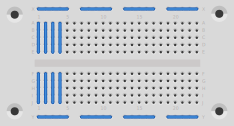
\includegraphics[align=c,width=0.2\textwidth]{./Graphics/breadboard}
    & 
    \begin{minipage}[t]{0.2\textwidth}
        \centering
        1 $\times$ Bread Board 
    \end{minipage}\\ \hline
    \includegraphics[align=c,width=0.2\textwidth]{./Graphics/150_resistor} 
    & 3 $\times$ 150$\Omega$ Resistor \\ \hline
    \includegraphics[align=c,width=0.2\textwidth]{./Graphics/rgb_led}
    & 1 $\times$ RGB LED \\ \hline
    \includegraphics[align=c,width=0.2\textwidth]{./Graphics/jumper_cables}
    & 4 $\times$ Jumper Cables \\ \hline
  \end{tabular}
\end{center}

\begin{center}
    \includegraphics[width=0.4\textwidth]{./Graphics/rgb_led_circuit}
\end{center}

The reason why you should use a resistor 
for every color is that 
\subsection{Hardware}

\begin{center}
    \includegraphics[height=0.2\textwidth]{./Graphics/rgb_internals}
\end{center}

A RGB LED can be thought of as 3 separate LEDs 
which happen to share a common ground 
in terms of a circuit.

\subsection{Pulse Width Modulation}
\begin{center}
    \includegraphics[height=0.4\textwidth]{./Graphics/pwd_mid}
\end{center}

The cycle for PWM is 2ms.
It varies between 0 and 255 
with 0 being fully off
and 255 being fully off.
Show in the diagram is somewhere around 64.

\subsection{Software}
\lstinputlisting[style=Arduino]{./Src/rgb.src}

random gives a random number between 0 and 255,
meaning any value for any channel from fully off
to fully on.
